\documentclass[11pt]{article}
\usepackage[margin=1.15in]{geometry}
\usepackage{amsmath,amssymb,amsthm}
\usepackage{booktabs,graphicx,microtype,setspace}
\usepackage[authoryear,round]{natbib}
\usepackage[colorlinks=true,linkcolor=black,citecolor=black,urlcolor=black]{hyperref}
\onehalfspacing
\newtheorem{proposition}{Proposition}
\newcommand{\R}{\mathbb{R}}
\title{Counting Edges and Counting Equations\\[4pt]\large What the Dimension-Matching Result Establishes, and What the Network Experiments Can and Cannot Confirm}
\author{Flyxion\\Independent Researcher}
\date{October 2026}
\begin{document}
\maketitle
\begin{abstract}
A recent paper on the modulatability of nonlinear oscillators poses an inverse problem: given desired values of oscillation properties such as period and amplitude, find parameters that produce them. Its central theoretical statement is that local uniqueness requires as many free parameters as target properties and a full-rank Jacobian, and its network experiments report that the number of edges that must be modulated matches the number of target nodes. The first statement is classical and correct. The second is a different kind of claim, and the way the experiment is assigned determines the diagonal on which it lands. This essay separates what the counting argument delivers from what it leaves open (rank, conditioning, locality, dependent properties), shows with a small model how the matched-dimension pattern follows from the assignment protocol and moves when propagation is present, and lists the baselines and checks that would make the empirical comparison with black-box optimizers decisive.
\end{abstract}

\section{The result and what is good about it}

Let $\mu\in\R^{\ell}$ collect adjustable parameters and let $\mathbf p(\mu)\in\R^{m}$ collect the oscillation properties of the limit cycle of $\dot x=f(x;\mu)$, for example period, amplitude, maximum and minimum of a coordinate. The inverse problem is to solve $\mathbf p(\mu)=\mathbf p^{\star}$. The paper's statement is that near a point $\mu_0$ the solution is locally unique when the Jacobian $J=\partial\mathbf p/\partial\mu$ is square ($m=\ell$) and nonsingular, by the inverse function theorem, and that the targets for which $J$ is singular form a set of measure zero in property space. The paper separates point, set and path modulatability, computes the Jacobian from a truncated Fourier representation of the orbit after a nonlinear time transformation, and follows solution paths by Newton continuation. It also notes that a maximum and a minimum are not independent properties of an oscillation, since they are $B+A$ and $B-A$ for offset $B$ and amplitude $A$, so that a nominal pair of targets may be one target twice. It identifies the failure of invertibility at path ends with saddle-node bifurcations of the orbit. These are real strengths: the formulation is explicit, the reparametrization of dependent properties shows care, and the continuation produces paths along which one property moves while another is held fixed.

None of what follows disputes these statements. The concern is with how far a dimension-counting statement can be carried when it is cited as the explanation for an experimental pattern, and with whether the comparison against baselines tests the claim it is taken to test.

\section{What dimension counting does not say}

\subsection{Count is necessary for a clean answer, rank is what matters}

Having $\ell=m$ parameters does not make the map locally invertible. It makes the Jacobian square, which is a precondition for asking whether it is invertible. A square $J$ can be singular everywhere on a set that is not small in the region of interest, for instance when two parameters enter only through a product, or when a property is insensitive to a parameter over a whole regime. Conversely, $\ell>m$ parameters is not an obstacle to a solution; it enlarges the solution set to a manifold of dimension $\ell-m$ when $J$ has rank $m$, which is exactly what the path-following part of the paper exploits. So the count says how many solutions to expect locally (zero-dimensional, or a manifold), and the rank says whether the count applies. The paper states both conditions; the issue is that downstream, ``dimension matching'' is used as shorthand for the first alone.

\subsection{Full rank is not well conditioned}

Local uniqueness is a qualitative property. Whether a solution can be found from a given starting point, and whether it survives parameter noise, depends on the size of the singular values of $J$ relative to the step sizes and tolerances in use. A simple illustration is the van der Pol oscillator $\ddot x-\mu(1-x^2)\dot x+\omega^2x=0$ with parameters $(\mu,\omega)$ and properties (period, amplitude). I computed the property map numerically and the log-sensitivity matrix by finite differences (script supplied). At $\omega=1$ the limit-cycle amplitude is close to $2$ for every nonlinearity in the range examined, and its logarithmic sensitivity to $\mu$ is small:
\begin{center}
\begin{tabular}{rrrrr}
\toprule
$\mu$ & amplitude & period & $\partial\log A/\partial\log\mu$ & ratio of singular values\\
\midrule
0.5 & 2.0025 & 6.381 & 0.0024 & 449\\
1.0 & 2.0086 & 6.663 & 0.0069 & 180\\
2.0 & 2.0199 & 7.630 & 0.0069 & 259\\
\bottomrule
\end{tabular}
\end{center}
The Jacobian with respect to $(\mu,\omega)$ is square and nonsingular at all three points, so the theorem applies. Yet to move the amplitude by a few percent through $\mu$ alone, a change of several orders of magnitude in $\mu$ would be required, so the solution is formally unique and practically inaccessible within any realistic parameter range. This is a property of a standard textbook system, not of a pathological one, and it indicates why modulatability regions in practice are bounded by sensitivity long before they are bounded by rank.

\subsection{Local existence only}

The inverse function theorem gives a neighborhood of $\mu_0$ on which $\mathbf p$ is a diffeomorphism onto a neighborhood of $\mathbf p(\mu_0)$. It does not say that a target outside that neighborhood is reachable, nor that it is unreachable. Global statements come from continuation, which the paper provides, but continuation inherits the limitation at every fold. The paper is candid that paths terminate at saddle-node bifurcations; the consequence is that set modulatability, the claim that a whole set of targets is reachable, is established numerically target by target rather than by the counting argument.

\subsection{Dependent properties}

When a property is a function of others, the effective $m$ is smaller than the nominal one. The paper handles the maximum and minimum case through the offset--amplitude parametrization. The general principle deserves emphasis: the relevant count is the rank of the map $\mu\mapsto\mathbf p$, and in a network with many nodes, node-wise amplitudes are coupled through the network, so that the effective number of independent targets can be below the number of targeted nodes. This matters for the next section.

\section{The matched-dimension pattern is produced by the protocol}

Figures 1g and 1h of the paper report, for gene-regulatory and FitzHugh--Nagumo networks, the fraction of target nodes whose amplitude changes by more than $\delta=0.05$ relative to baseline, as a function of the number of targets $m_{\rm target}$ and the number of modulated edges $m_{\rm edge}$, with a high success rate along the diagonal $m_{\rm edge}\approx m_{\rm target}$. The Methods describe the assignment as follows. A random permutation of the nodes is drawn; the first $m_{\rm target}$ nodes are the targets and the first $m_{\rm edge}$ nodes are the recipients of a perturbation; each recipient receives one incoming edge whose weight is increased by a fixed $\Delta w$ ($0.03$ for the gene-regulatory model, $0.3$ for the FHN model). When $m_{\rm edge}\ge m_{\rm target}$ every target gets one perturbation and the remainder go to non-targets; when $m_{\rm edge}<m_{\rm target}$ only the first $m_{\rm edge}$ targets are directly perturbed and the rest are affected through propagation only. Trials without a post-modulation periodic orbit are omitted, and success is threshold exceedance, not attainment of a specified value.

Three features of this design bear on interpretation.

\paragraph{The diagonal is a consequence of the assignment rule.} Because the ordering puts targets first, a target is perturbed directly if and only if its index is below $m_{\rm edge}$. Direct perturbation of a node by a fixed increment will move its amplitude by an amount that depends on its sensitivity, and the paper's $\delta=0.05$ is a threshold the direct effect often exceeds. So the success fraction at $(m_{\rm target},m_{\rm edge})$ is roughly $\min(1,m_{\rm edge}/m_{\rm target})$ plus whatever propagation contributes. That is a ridge on the diagonal before any appeal to the Jacobian.

\paragraph{The edges are not chosen to hit a target.} The edge increments are fixed and random, and success is exceedance of a threshold. This tests whether a random fixed perturbation moves a node by more than $\delta$, which is a question about sensitivity and about propagation, and is different from the inverse problem the theorem addresses: find a $\Delta w$ that produces a prescribed amplitude. A square nonsingular Jacobian is neither necessary nor sufficient for the heatmap pattern.

\paragraph{Propagation changes where the ridge lies.} The paper acknowledges that unperturbed targets are affected through propagation. If propagation is strong, targets without a direct perturbation also exceed the threshold, and the ridge moves to $m_{\rm edge}<m_{\rm target}$. The location of the diagonal therefore depends on coupling strength and graph structure, which are properties of the system, and on $\Delta w$ and $\delta$, which are properties of the protocol.

To see how large this effect can be, I built a deliberately crude toy (supplied as \texttt{modul.py}): $n=100$ nodes on an Erd\H{o}s--R\'enyi graph of mean degree $6$; a directly perturbed node changes its amplitude by $0.08$ (above $\delta=0.05$); each perturbed in-neighbor adds $g\times0.08$ to a node's change. Assignment follows the same targets-first rule, with $60$ trials per cell. For $m_{\rm target}=50$, the smallest $m_{\rm edge}$ at which the mean success fraction reaches $0.9$ is
\begin{center}
\begin{tabular}{lccc}
\toprule
propagation gain $g$ & $0$ & $0.3$ & $0.9$\\
\midrule
smallest $m_{\rm edge}$ for success $\ge0.9$ & 46 & 41 & 26\\
\bottomrule
\end{tabular}
\end{center}
With no propagation the ridge sits at the diagonal, as the protocol dictates; with strong propagation about half as many edges suffice. Figure~\ref{fig:modul} shows the three heatmaps. The toy is not a model of either network in the paper and its numbers should not be read as predictions for them. It shows only that the diagonal can be produced by the rule that places targets first, and that its position is not a fixed consequence of a dimension count.

\begin{figure}[t]
\centering
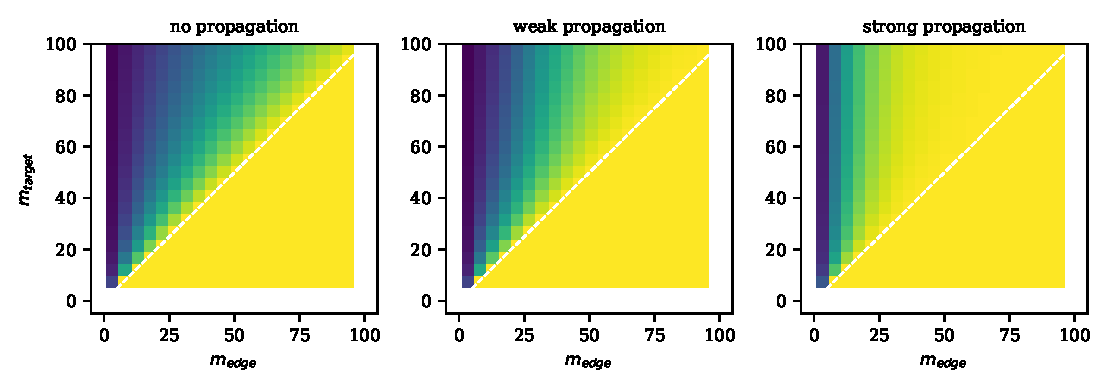
\includegraphics[width=\textwidth]{fig_modul.pdf}
\caption{Toy success-rate heatmaps under the targets-first assignment rule, for no, weak and strong propagation. The dashed line is $m_{\rm edge}=m_{\rm target}$. With $g=0$ the ridge lies on the line by construction; with $g=0.9$ it lies well below it.}
\label{fig:modul}
\end{figure}

The sweeping experiments in the paper (other topologies, sizes, target-selection strategies and thresholds, in its supplement, which I have not read) are a step in the right direction. The check that matters most is whether the diagonal survives when targets are chosen adversarially, for example as nodes with low in-degree or low sensitivity, since in that case the targets-first alignment between directly perturbed and targeted nodes no longer helps.

\section{The comparison with black-box optimizers}

The paper compares its Newton-continuation method with uniform random sampling, quasi-random sampling, particle swarm optimization and Powell's method, under a fixed search budget, and reports lower error and smaller failure rates for its method. This is a reasonable comparison for the stated purpose of showing that a model-informed method beats model-free search. It leaves three questions open.

\paragraph{Information asymmetry.} The proposed method uses derivatives of the orbit, obtained from the model's equations. The baselines listed use function values only. A comparison that includes the same derivative information is the comparison that isolates the contribution of the Fourier-and-continuation machinery from the contribution of using gradients at all. The natural controls are Gauss--Newton or Levenberg--Marquardt on the same property residual, with finite-difference or adjoint Jacobians, and multistart versions of each. If the proposed method wins against these, the contribution is the orbit parametrization and continuation; if it ties, the contribution is mainly the use of gradients.

\paragraph{What counts as a failure and what a trial costs.} The Newton method needs a periodic-orbit solve at each step, which is expensive compared with a function evaluation for a derivative-free optimizer. A fixed number of function evaluations is a different budget from a fixed wall-clock time. The informative summary is time to success over all trials, including failed ones, with the failure criterion stated in advance. The treatment of trajectories that leave the oscillatory regime (omitted in the heatmaps, as the Methods state) should be reported in the same way for every method.

\paragraph{Where targets come from.} Targets drawn by perturbing a known parameter and recording the properties are guaranteed reachable; targets drawn uniformly from a box in property space may not be. The difficulty of the benchmark depends on which, and results should state it.

\section{Checks that would settle it}

\begin{enumerate}
\item Randomize the assignment of recipients independently of the target set, and report the heatmap against both $m_{\rm edge}$ and the number of targets with at least one direct incoming perturbation.
\item Vary $\Delta w$ and $\delta$ over a wide range, and report whether the ridge position moves, as the toy suggests it should if propagation matters.
\item Replace threshold exceedance by attainment of prescribed amplitudes (equality targets) and solve for $\Delta w$ by the method; report success against $m_{\rm edge}-m_{\rm target}$.
\item Report the singular values of $J$ along every path, so that near-singularity before a bifurcation is visible, and report the condition number of the problem at the start and at the end.
\item Add Levenberg--Marquardt and multistart Gauss--Newton baselines on the same residual, and report time to success including failures.
\end{enumerate}

\section{Conclusion}
\nocite{hirsch,nw,strogatz}

The theoretical statement is correct and carefully qualified: a square, full-rank Jacobian gives local uniqueness, and the exceptional targets are a null set. The paper's own treatment of dependent properties and of bifurcations shows that its authors know where the statement stops. What the statement does not do is explain a diagonal in an experiment whose assignment rule places targets first and perturbs them one-for-one, because that diagonal can be produced without any appeal to rank, and moves when propagation is present. Nor does a comparison with derivative-free optimizers show that the orbit parametrization, as opposed to derivative information, is what helps. The method may well be better; the checks above would show whether and why.

\paragraph{Limits of this essay.} The paper's supplement was not read. The van der Pol computation and the network toy are illustrations of mechanisms, not reproductions of any result in the paper, and the toy's parameters were chosen for clarity.

\begin{thebibliography}{9}
\bibitem[Hirsch et al.(2013)]{hirsch} Hirsch, M.~W., Smale, S.\ and Devaney, R.~L.\ (2013). \emph{Differential Equations, Dynamical Systems, and an Introduction to Chaos}, 3rd edn. Academic Press.
\bibitem[Nocedal and Wright(2006)]{nw} Nocedal, J.\ and Wright, S.~J.\ (2006). \emph{Numerical Optimization}, 2nd edn. Springer.
\bibitem[Strogatz(2015)]{strogatz} Strogatz, S.~H.\ (2015). \emph{Nonlinear Dynamics and Chaos}, 2nd edn. Westview Press.
\end{thebibliography}
\end{document}
